% Beamer's default font size is 11 points. It is possible to set the
% default font size to any of 8, 9, 10, 11, 12, 14, 17, 20
\documentclass[13pt]{beamer}

\usetheme{Warsaw}
%\usecolortheme{dolphin}
\usecolortheme{seahorse}
%\useinnertheme{circles}
\usefonttheme{professionalfonts}
%\usefonttheme{structurebold}
%\usefonttheme{default} 
\setbeamertemplate{navigation symbols}{}
\usepackage[english]{babel}
\usepackage[latin1]{inputenc}
\usepackage{times}
\usepackage[T1]{fontenc}

% These things can change:
\newcommand{\baseurl}{http://cell.vtt.fi/latex}
\urlstyle{sf}

\begin{document}

\logo{
\includegraphics[width=1.4cm]{img/vttplain}\quad}
\title{\scalebox{1.5}{\textrm{\LaTeX}} Course 2011}
\subtitle{Part 1: Short Introduction}
\author{Arho Virkki}
\institute{\textsc{VTT Technical Research Centre of Finland}}
\date{}

\begin{frame}
  \titlepage
\end{frame}

\begin{frame}\frametitle{\LaTeX{}--distribution packages}
The very same \LaTeX{} in different packages:\medskip

\begin{itemize}
\item TeXLive (Linux, Mac OS X, Windows)
\item MacTeX (Mac OS X)
\item MikTeX (Windows)
\item \dots
\end{itemize}
\end{frame}

\begin{frame}\frametitle{\LaTeX{} on Ubuntu Linux through Synaptic}
\includegraphics[width=0.92\textwidth]{img/Synaptic_TeXLive}
\end{frame}

\begin{frame}\frametitle{\LaTeX{} on Mac OS X}
\qquad\includegraphics[width=0.75\textwidth]{img/MacTeX_install}
\end{frame}

\begin{frame}\frametitle{\LaTeX{} on Windows}
\qquad\includegraphics[width=0.75\textwidth]{img/MiKTeX}\medskip

\url{http://miktex.org/2.9/setup}
\end{frame}


\begin{frame}[fragile]\frametitle{Document structure}
An example document preamble:
{\small
\begin{verbatim}
\documentclass[a4paper,10pt]{article} % style
\usepackage[latin1]{inputenc} % or [ansinew]
\usepackage[finnish]{babel}   % hyphenation
\usepackage{graphicx}         % for images

\begin{document}
\section{Introduction}
During the last few decades, the amount of digital
content has increased enormously
\dots
\end{document}
\end{verbatim}
}
\end{frame}


\begin{frame}[fragile]\frametitle{Compilation: Linux \& Mac command line}

Just call LaTeX or PDFLaTeX directly 
{\small
\begin{verbatim}
$ latex myfile.tex; dvipdf myfile  # or
$ pdflatex myfile                           
\end{verbatim}}\medskip

and then inspect the content:
{\small
\begin{verbatim}
$ gnome-open myfile.pdf # Linux
$ open myfile.pdf       # Mac                           
\end{verbatim}}\medskip

\end{frame}


\begin{frame}\frametitle{Compilation: Windows}
{\small Point and click - depending on the chosen interface}\bigskip

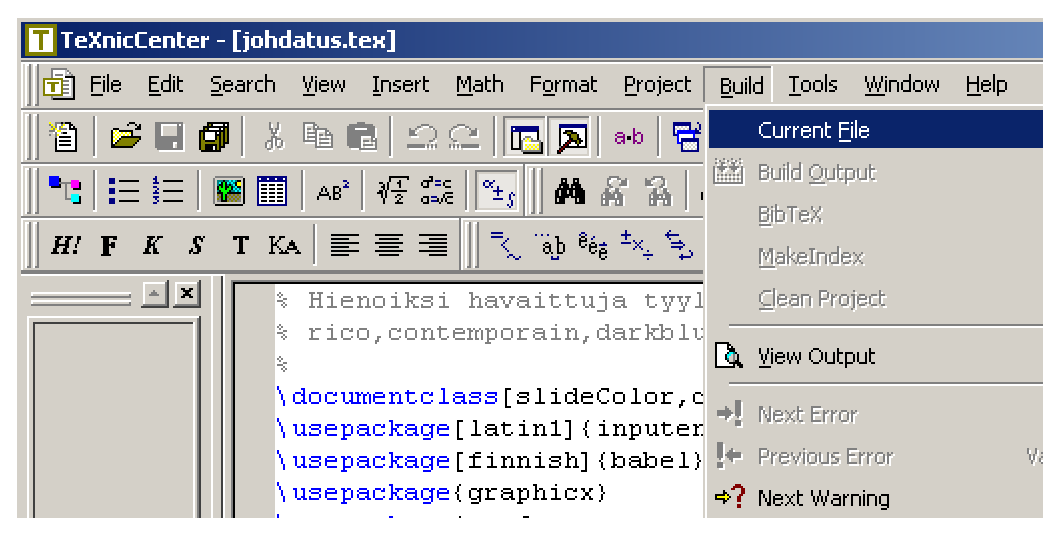
\includegraphics[width=0.8\textwidth]{img/texniccenter}
\end{frame}


\begin{frame}[fragile]\frametitle{Mathematics}
Equations are written between the \$ -characters. For example, 
\begin{center}
\verb|$\sqrt{x^3}$| $\qquad\mapsto\qquad \sqrt{x^3}$
\end{center}
or separately as
\begin{verbatim}
   \[  \sqrt{x^3}  \]
\end{verbatim}
or using 
\begin{verbatim}
   \begin{equation}
   \sqrt{x^3}
   \end{equation}
\end{verbatim}
where the latter gives the equation also a number.
\end{frame}


\begin{frame}[fragile]\frametitle{Mathematics\ldots}
Examples: \\
{\small
\begin{verbatim}
\begin{equation}\label{eq:gammaf}
  \Gamma (n) := 
  \int_0^\infty x^{n-1}e^{-x} dx 
\end{equation}
Observe that (\ref{eq:gammaf}) does not converge
when $n=0$
\end{verbatim}
\begin{equation}
  \Gamma (n) := 
  \int_0^\infty x^{n-1} e^{-x} dx
\end{equation}
Observe that (1) does not converge 
when $n=0$.}
\end{frame}


\begin{frame}[fragile]\frametitle{Mathematics\dots}
{\small
\begin{verbatim}
\[ \neg A := X \setminus A \]
\end{verbatim} 

\[ \neg A := X \setminus A \]

\begin{verbatim}
\[ \zeta(s) := 
   \sum_{k=1}^\infty \frac{1}{k^s} \]
\end{verbatim}

\[ \zeta(s) := \sum_{k=1}^\infty \frac{1}{k^s} \]
}
\end{frame}


\begin{frame}[fragile]\frametitle{Mathematics\dots}
It is best to learn the basic commands  
\begin{verbatim}
\frac{}{}
\int
\sum
\dots
\end{verbatim}
by heart. There are just a few of them and they are rather logical.\bigskip

(Observe  that \verb|\int| = integral, not an integer\dots)
\end{frame}


\begin{frame}[fragile]\frametitle{Structures}
Structures define how the text is displayed.\medskip

Examples: \\
{\small
\begin{verbatim}
\begin{enumerate}
\item Firstly,
\item Secondly\dots
\end{enumerate}
\end{verbatim}\bigskip

\begin{enumerate}
\item Firstly,
\item Secondly\dots
\end{enumerate}
}
\end{frame}


\begin{frame}[fragile]\frametitle{Structures\dots}
{\small
\begin{verbatim}
\begin{itemize}
\item gloves
\item shoes
\end{itemize}
\end{verbatim}\bigskip

\begin{itemize}
\item gloves
\item shoes
\end{itemize}
}
\end{frame}


\begin{frame}[fragile]\frametitle{Structures\dots}
{\footnotesize
\begin{verbatim}
My maths teaches was a genius to explain things:
\begin{quote} 
We define the determinant like a civil service 
department would, in a rather boring way: It is just 
thrown to your face with the motivation being 
"learn it or die".
\end{quote}
\end{verbatim}}

My maths teaches was a genius to explain things:
\begin{quote} 
We define the determinant like a civil service 
department would, in a rather boring way: It is just 
thrown to your face with the motivation being 
"learn it or die".
\end{quote}
\end{frame}


\begin{frame}[fragile]\frametitle{Graphics}
In \LaTeX, everything can be thought of being composed of boxes,
aligned with respect to each other, and the distances between them.\medskip

Examples: \\[1em]
{\small
\begin{minipage}{0.6\textwidth}
\begin{verbatim}
\begin{center}
\fbox{
\rotatebox{-30}{
\fbox{

\includegraphics[width=2cm]
{/img/vttplain}}}}
\vspace*{1cm}
\end{verbatim}
\end{minipage}
\begin{minipage}{0.39\textwidth}
\begin{center}
\fbox{
\rotatebox{-30}{
\fbox{

\includegraphics[width=2cm]{img/vttplain}
}}}
\end{center}
\end{minipage}
}
\end{frame}


\begin{frame}[fragile]\frametitle{Graphics\dots}
{\small
\begin{minipage}{0.6\textwidth}
\begin{verbatim}
\reflectbox{
\rotatebox{30}{
\resizebox{!}{5mm}{Tricky stuff}
}}

\vspace*{1cm}
\rule{3cm}{1ex}
\end{verbatim}
\end{minipage}
\begin{minipage}{0.39\textwidth}
\begin{center}
\reflectbox{
\rotatebox{30}{
\resizebox{!}{5mm}{Tricky stuff}
}}

\vspace*{1cm}
\rule{3cm}{1ex}
\end{center}
\end{minipage}
}
\end{frame}


\begin{frame}[fragile]\frametitle{Summary}
\begin{itemize}
  \item The LaTeX manuscript file consists of plain text. It takes only a 
  little amount of disk space and it is simple to send to others.
  \item The manuscript always begins with the
  ``\verb|\documentclass[<params>]{<class>}|'' command\footnote{I suggest to
  copy the preamble from an existing template.\\ Try to avoid the ancient 
  templates from the early 80's, as things have changes since that.}.
\item The text consists of the commands (called tags in HTML) and the actual
  text.
\item This is not harder that writing HTML5 / CSS3 by hand. To be honest,
LaTeX is much easier!
\end{itemize}
\end{frame}

\end{document}
